\documentclass[12pt,a4paper]{article}
\usepackage[utf8]{vietnam}
\usepackage{amsmath,amssymb}
\usepackage{tabularx}
\usepackage{graphicx}
\usepackage{tikz}
\usetikzlibrary{calc,arrows.meta}
\usepackage{xcolor}
\usepackage{enumitem}
\usepackage{fancyhdr}
\usepackage[top=0.8cm, bottom=0.8cm, left=1.2cm, right=1.2cm]{geometry}
\usepackage[dethi]{ex_test}
\SAOPTN{widthSA=2.6,heightSA=0.62}

\setlength{\headheight}{15pt}
\setlength{\parskip}{0pt}

\pagestyle{fancy}
\fancyhf{}
\rhead{\textit{Môn Toán 7 -- Đề số 12}}
\lhead{\textit{Bộ đề ôn tập Giữa học kì I}}
\cfoot{\thepage}

\begin{document}

% --- KHUNG TIÊU ĐỀ ĐỀ THI ---
\noindent
\begin{tabularx}{\linewidth}{X r}
\textbf{TRƯỜNG THCS: \dotfill} & \textbf{ĐỀ KIỂM TRA ĐỊNH KỲ GIỮA HỌC KỲ I} \\
\textbf{Họ và tên: \dotfill} & \textbf{NĂM HỌC 2026 -- 2027} \\
\textbf{Lớp: \dotfill \quad SBD: \dotfill} & \textbf{Môn: TOÁN 7} \\
& \textit{Thời gian làm bài: 90 phút (không kể thời gian phát đề)}
\end{tabularx}

\vspace{1mm}
\noindent
\begin{tabularx}{\linewidth}{|p{3.5cm}|X|}
\hline
\centering\textbf{Điểm số} & \centering\textbf{Lời nhận xét của thầy cô giáo} \tabularnewline
\rule{0pt}{0.8cm} & \\
\hline
\end{tabularx}

\vspace{1.5mm}
\begin{center}
\textbf{\large ĐỀ SỐ 12}
\end{center}

\noindent\textbf{\large PHẦN I. CÂU TRẮC NGHIỆM NHIỀU PHƯƠNG ÁN LỰA CHỌN (3,0 điểm)}

\textit{Thí sinh trả lời từ câu 1 đến câu 12. Mỗi câu hỏi chỉ chọn một phương án đúng nhất và ghi vào bảng đáp án.}

\vspace{1mm}
\begin{ex}
Kết quả của phép tính $-\dfrac{7}{8} - \dfrac{5}{4}$ là:
\choice
{$\dfrac{3}{8}$}
{$\dfrac{17}{8}$}
{$-\dfrac{3}{8}$}
{\True $-\dfrac{17}{8}$}
\end{ex}

\begin{ex}
Các mặt bên của hình lăng trụ đứng tam giác là:
\choice
{Các hình tam giác}
{\True Các hình chữ nhật}
{Các hình thang cân}
{Các hình vuông}
\end{ex}

\begin{ex}
Một hình lập phương có cạnh $a = 5\text{ cm}$. Diện tích xung quanh của hình lập phương đó là:
\choice
{$25\text{ cm}^2$}
{$50\text{ cm}^2$}
{\True $100\text{ cm}^2$}
{$150\text{ cm}^2$}
\end{ex}

\begin{ex}
Trong các số sau, số nào là số vô tỉ?
\choice
{$\sqrt{9}$}
{$\dfrac{3}{2}$}
{$2{,}5$}
{\True $\sqrt{5}$}
\end{ex}

\begin{ex}
\immini{
Cho hình lăng trụ đứng tam giác $ABC.A'B'C'$ (như hình vẽ bên). Các mặt bên của hình trên là những hình gì?
\choice
{Tam giác}
{Hình thoi}
{\True Hình chữ nhật}
{Hình bình hành}
}{
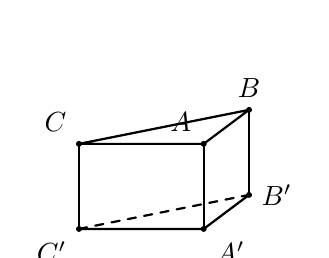
\begin{tikzpicture}[scale=0.72, line cap=round, line join=round]
    \coordinate (C) at (0, 1.5);
    \coordinate (A) at (2.2, 1.5);
    \coordinate (B) at (3.0, 2.1);
    \coordinate (C_prime) at (0, 0);
    \coordinate (A_prime) at (2.2, 0);
    \coordinate (B_prime) at (3.0, 0.6);

    \draw[thick] (C) -- (A) -- (B) -- (C);
    \draw[thick] (C) -- (C_prime);
    \draw[thick] (A) -- (A_prime);
    \draw[thick] (B) -- (B_prime);
    \draw[thick] (C_prime) -- (A_prime) -- (B_prime);
    \draw[thick, dashed] (C_prime) -- (B_prime);

    \filldraw[black] (C) circle (1.2pt) node[above left=1pt] {$C$};
    \filldraw[black] (A) circle (1.2pt) node[above left=1pt] {$A$};
    \filldraw[black] (B) circle (1.2pt) node[above=1pt] {$B$};
    \filldraw[black] (C_prime) circle (1.2pt) node[below left=1pt] {$C'$};
    \filldraw[black] (A_prime) circle (1.2pt) node[below right=1pt] {$A'$};
    \filldraw[black] (B_prime) circle (1.2pt) node[right=1pt] {$B'$};
\end{tikzpicture}
}
\end{ex}

\begin{ex}
Số nào trong các số dưới đây không là số hữu tỉ?
\choice
{\True $\dfrac{3}{0}$}
{$0{,}625$}
{$\dfrac{0}{3}$}
{$2\dfrac{3}{5}$}
\end{ex}

\begin{ex}
Tích $(-3{,}1) \cdot (-3{,}1) \cdot (-3{,}1) \cdot (-3{,}1) \cdot (-3{,}1)$ viết gọn là:
\choice
{$(-3{,}1) \cdot 5$}
{\True $(-3{,}1)^5$}
{$(3{,}1)^5$}
{$3{,}1 \cdot 5$}
\end{ex}

\begin{ex}
Kết quả của phép tính $\dfrac{4}{7} - \dfrac{5}{9}$ bằng:
\choice
{\True $\dfrac{1}{63}$}
{$\dfrac{2}{63}$}
{$\dfrac{4}{63}$}
{$\dfrac{5}{63}$}
\end{ex}

\newpage
\begin{ex}
\immini{
Cho điểm $O$ thuộc đường thẳng $AB$. Số đo $\widehat{BOC}$ trong hình vẽ bên là:
\choice
{\True $60^\circ$}
{$120^\circ$}
{$180^\circ$}
{$90^\circ$}
}{
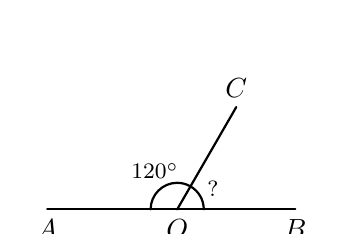
\begin{tikzpicture}[scale=0.75, line cap=round, line join=round]
    \coordinate (O) at (0,0);
    \coordinate (A) at (-2.2,0);
    \coordinate (B) at (2.0,0);
    \coordinate (C) at (60:2.0);
    \draw[thick] (A) -- (B);
    \draw[thick] (O) -- (C);
    \node[below] at (A) {$A$};
    \node[below] at (O) {$O$};
    \node[below] at (B) {$B$};
    \node[above] at (C) {$C$};
    \draw[thick] (O) ++(180:0.45) arc (180:60:0.45);
    \node[font=\footnotesize] at (120:0.75) {$120^\circ$};
    \draw[thick] (O) ++(60:0.45) arc (60:0:0.45);
    \node[font=\footnotesize] at (30:0.7) {$?$};
\end{tikzpicture}
}
\end{ex}

\begin{ex}
Số nào dưới đây là số thập phân vô hạn tuần hoàn?
\choice
{$0{,}123123$}
{$\dfrac{1}{2}$}
{\True $0{,}(3)$}
{$0{,}3$}
\end{ex}

\begin{ex}
Cho $\widehat{xOy} = 70^\circ$. Góc đối đỉnh với $\widehat{xOy}$ có số đo bằng:
\choice
{$110^\circ$}
{\True $70^\circ$}
{$180^\circ$}
{$35^\circ$}
\end{ex}

\begin{ex}
Một hình hộp chữ nhật có chiều dài $6\text{ cm}$, chiều rộng $4\text{ cm}$ và chiều cao $5\text{ cm}$. Thể tích của hình hộp chữ nhật đó là:
\choice
{\True $120\text{ cm}^3$}
{$74\text{ cm}^3$}
{$60\text{ cm}^3$}
{$120\text{ cm}^2$}
\end{ex}


\vspace{1mm}
\noindent\textbf{BẢNG TRẢ LỜI TRẮC NGHIỆM PHẦN I:}
\begin{center}
\begin{tabular}{|c|c|c|c|c|c|c|c|c|c|c|c|c|}
\hline
\textbf{Câu} & \textbf{1} & \textbf{2} & \textbf{3} & \textbf{4} & \textbf{5} & \textbf{6} & \textbf{7} & \textbf{8} & \textbf{9} & \textbf{10} & \textbf{11} & \textbf{12} \\
\hline
\textbf{Chọn} & \rule{0pt}{0.48cm} & & & & & & & & & & & \\
\hline
\end{tabular}
\end{center}
\vspace{1mm}

\setcounter{ex}{0}
\noindent\textbf{\large PHẦN II. CÂU TRẮC NGHIỆM ĐÚNG SAI (2,0 điểm)}

\textit{Thí sinh trả lời câu 1 và câu 2. Trong mỗi ý a), b), c), d) ở mỗi câu, thí sinh chọn đúng hoặc sai.}

\vspace{1mm}
\begin{ex}
Cho biểu thức $X = \left(-\dfrac{3}{2}\right)^2 - \dfrac{5}{4} \cdot \left(-\dfrac{2}{5}\right) + \left(-\dfrac{1}{4}\right)$. Xét tính đúng sai của các mệnh đề sau:
\choiceTF
{\True Giá trị của lũy thừa $\left(-\dfrac{3}{2}\right)^2$ bằng $\dfrac{9}{4}$}
{\True Giá trị của phép nhân $\dfrac{5}{4} \cdot \left(-\dfrac{2}{5}\right)$ bằng $-\dfrac{1}{2}$}
{Giá trị của biểu thức $X$ bằng $3$}
{Giá trị $X$ thu được là một số nguyên âm}
\end{ex}

\begin{ex}
\immini{
Quan sát hình lăng trụ đứng tam giác $ABC.A'B'C'$ dưới đây. Xét tính đúng sai của các mệnh đề sau:
\choiceTF
{\True Hai mặt đáy của hình lăng trụ đứng là tam giác $ABC$ và tam giác $A'B'C'$}
{Các mặt bên $ABB'A', BCC'B', ACC'A'$ là các hình tam giác}
{\True Các cạnh bên $AA', BB', CC'$ song song và bằng nhau}
{\True Nếu đáy $ABC$ là tam giác vuông tại $A$ có $AB = 3\text{ cm}, AC = 4\text{ cm}$ và chiều cao $AA' = 5\text{ cm}$ thì thể tích của hình lăng trụ bằng $30\text{ cm}^3$}
}{
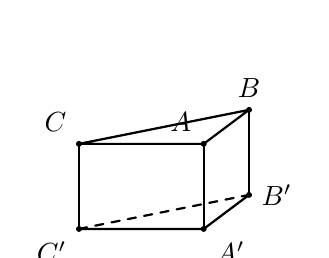
\begin{tikzpicture}[scale=0.72, line cap=round, line join=round]
    \coordinate (C) at (0, 1.5);
    \coordinate (A) at (2.2, 1.5);
    \coordinate (B) at (3.0, 2.1);
    \coordinate (C_prime) at (0, 0);
    \coordinate (A_prime) at (2.2, 0);
    \coordinate (B_prime) at (3.0, 0.6);

    \draw[thick] (C) -- (A) -- (B) -- (C);
    \draw[thick] (C) -- (C_prime);
    \draw[thick] (A) -- (A_prime);
    \draw[thick] (B) -- (B_prime);
    \draw[thick] (C_prime) -- (A_prime) -- (B_prime);
    \draw[thick, dashed] (C_prime) -- (B_prime);

    \filldraw[black] (C) circle (1.2pt) node[above left=1pt] {$C$};
    \filldraw[black] (A) circle (1.2pt) node[above left=1pt] {$A$};
    \filldraw[black] (B) circle (1.2pt) node[above=1pt] {$B$};
    \filldraw[black] (C_prime) circle (1.2pt) node[below left=1pt] {$C'$};
    \filldraw[black] (A_prime) circle (1.2pt) node[below right=1pt] {$A'$};
    \filldraw[black] (B_prime) circle (1.2pt) node[right=1pt] {$B'$};
\end{tikzpicture}
}
\end{ex}


\noindent\textbf{BẢNG TRẢ LỜI PHẦN II:}
\begin{center}
\begin{tabular}{|c|c|c|c|c||c|c|c|c|c|}
\hline
\textbf{Câu 1} & \textbf{a)} & \textbf{b)} & \textbf{c)} & \textbf{d)} & \textbf{Câu 2} & \textbf{a)} & \textbf{b)} & \textbf{c)} & \textbf{d)} \\
\hline
\textbf{Đ/S} & \rule{0pt}{0.45cm} & & & & \textbf{Đ/S} & & & & \\
\hline
\end{tabular}
\end{center}
\vspace{1mm}

\setcounter{ex}{0}
\noindent\textbf{\large PHẦN III. CÂU HỎI TRẢ LỜI NGẮN (1,0 điểm)}

\textit{Thí sinh trả lời câu 1 và câu 2. Điền kết quả vào ô trống.}

\vspace{1mm}
\begin{ex}
Tìm số tự nhiên $x$, biết: $3^{x+2} - 3^x = 216$. \shortans{3}
\end{ex}

\begin{ex}
Cho hai đường thẳng song song $a$ và $b$. Đường thẳng $c$ cắt $a$ và $b$ lần lượt tại hai điểm $A$ và $B$. Biết $\widehat{A}_1$ và $\widehat{B}_1$ là hai góc trong cùng phía và $\widehat{A}_1 = 2\widehat{B}_1$. Tính số đo góc $\widehat{A}_1$. \shortans{$120^\circ$}
\end{ex}


\newpage
\setcounter{ex}{0}
\noindent\textbf{\large PHẦN IV. TỰ LUẬN (4,0 điểm)}

\textit{Thí sinh trình bày chi tiết lời giải vào giấy làm bài.}

\vspace{1mm}
\begin{ex}
Tính hợp lý (nếu có):
\begin{enumerate}[label=\textbf{\alph*)}, leftmargin=0.8cm, itemsep=1pt]
\item $\dfrac{1}{6} - \dfrac{2}{5}$
\item $\left(-\dfrac{1}{3}\right)^2 : \dfrac{5}{9} + (-1)^{2024}$
\item $\left(\dfrac{5}{171} + \dfrac{8}{3}\right) - \left(-\dfrac{5}{3} - \dfrac{5}{171}\right) - 1\dfrac{2}{5}$
\end{enumerate}
\end{ex}
\vspace{2mm}

\begin{ex}
Tìm $x$, biết:
\begin{enumerate}[label=\textbf{\alph*)}, leftmargin=0.8cm, itemsep=1pt]
\item $\dfrac{1}{3} + \dfrac{2}{3} : x = -7$
\item $(x - 2{,}5)^2 = 16$
\end{enumerate}
\end{ex}
\vspace{2mm}

\begin{ex}
\immini{
Cho hình vẽ bên, trong đó $Ax \parallel By$ và $\widehat{xAB} = 40^\circ, \widehat{ABC} = 105^\circ, \widehat{BCz} = 65^\circ$.
\begin{enumerate}[label=\textbf{\alph*)}, leftmargin=0.8cm, itemsep=1pt]
\item Tính số đo $\widehat{ABy}$.
\item Chứng minh rằng $By$ song song với $Cz$.
\item Kẻ $BD$ là tia phân giác của $\widehat{CBy}$ ($D \in Cz$). Tính số đo $\widehat{BDC}$.
\end{enumerate}
}{
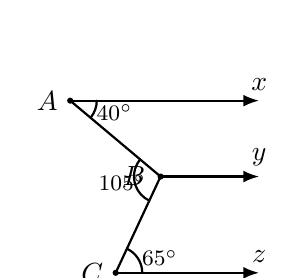
\begin{tikzpicture}[scale=0.75, line cap=round, line join=round]
    \coordinate (A) at (0, 2.4);
    \coordinate (x) at (3.2, 2.4);
    \coordinate (B) at (1.53, 1.115);
    \coordinate (y) at (3.2, 1.115);
    \coordinate (C) at (0.77, -0.515);
    \coordinate (z) at (3.2, -0.515);

    \draw[thick, -{Latex[length=2mm]}] (A) -- (x) node[above] {$x$};
    \draw[thick, -{Latex[length=2mm]}] (B) -- (y) node[above] {$y$};
    \draw[thick, -{Latex[length=2mm]}] (C) -- (z) node[above] {$z$};
    \draw[thick] (A) -- (B) -- (C);

    \filldraw[black] (A) circle (1.2pt) node[left=1pt] {$A$};
    \filldraw[black] (B) circle (1.2pt) node[left=2pt] {$B$};
    \filldraw[black] (C) circle (1.2pt) node[left=1pt] {$C$};

    % Angles
    \draw[thick] (A) ++(0:0.45) arc (0:-40:0.45);
    \node[font=\footnotesize] at ($(A)+(0.75,-0.2)$) {$40^\circ$};

    \draw[thick] (B) ++(140:0.45) arc (140:245:0.45);
    \node[font=\footnotesize] at ($(B)+(-0.65,-0.1)$) {$105^\circ$};

    \draw[thick] (C) ++(0:0.45) arc (0:65:0.45);
    \node[font=\footnotesize] at ($(C)+(0.75,0.25)$) {$65^\circ$};
\end{tikzpicture}
}
\end{ex}
\vspace{2mm}

\begin{ex}
Vào tháng 4, giá niêm yết của một chiếc laptop tại một cửa hàng máy tính là $16\,000\,000$ đồng. Đến tháng 8, cửa hàng giảm giá $10\%$ cho mỗi chiếc laptop. Sang tháng 10, cửa hàng lại giảm giá thêm một lần nữa, lúc này giá một chiếc laptop chỉ còn $13\,680\,000$ đồng. Hỏi tháng 10 cửa hàng đã giảm giá bao nhiêu phần trăm cho một chiếc laptop so với tháng 8?
\end{ex}
\vspace{2mm}


\begin{center}
\rule{4cm}{0.4pt}\\
\textit{--- HẾT ---}
\end{center}
\end{document}
